\documentclass{beamer}
\usepackage{beamerthemeshadow}

%\documentclass{article}
%\usepackage{beamerarticle}
%\usepackage{graphicx}

\usepackage{verbatim}
%\usepackage{lastpage}
\usepackage{xcolor}
\usepackage{pgf}
\usepackage{colortbl}

\newcommand{\bi}{\begin{itemize}}
\newcommand{\ei}{\end{itemize}}
\newcommand{\be}{\begin{enumerate}}
\newcommand{\ee}{\end{enumerate}}
\newcommand{\bd}{\begin{description}}
\newcommand{\ed}{\end{description}}
\newcommand{\prbf}[1]{\textbf{#1}}
\newcommand{\prit}[1]{\textit{#1}}
\newcommand{\beq}{\begin{equation}}
\newcommand{\eeq}{\end{equation}}
\newcommand{\bdm}{\begin{displaymath}}
\newcommand{\edm}{\end{displaymath}}

\newcommand{\ft}[1]{
  \frametitle{\begin{tabular}{p{4.2in}r} \textcolor{white}{#1} & \small{\insertframenumber / \inserttotalframenumber} \end{tabular}}
  %\frametitle{#1}
  \setbeamercovered{transparent=18}
}

\newcommand{\stepinv}{\setbeamercovered{invisible}}
\newcommand{\stopinv}{\setbeamercovered{transparent=18}}
\newcommand{\uncoverinv}[1]
{
  \setbeamercovered{invisible}
  \uncover<+->{#1}
  \setbeamercovered{transparent=18}
}
\newcommand{\ans}[1]{\textcolor{blue}{#1}}
\newcommand{\ansinv}[1]
{
  \setbeamercovered{invisible}
  \uncover<+->{\textcolor{blue}{#1}}
  \setbeamercovered{transparent=18}
}
\newcommand{\setinv}{\setbeamercovered{invisible}}
\newcommand{\setvis}{\setbeamercovered{transparent=18}}
\newcommand{\centerpic}[2]
{
  \begin{center}
  \includegraphics[#1]{#2}
  \end{center}
}
\newcommand{\h}[1]{\hat{#1}}
\newcommand{\ds}{\displaystyle}

%\definecolor{light}{rgb}{0.17,0.55,0.35}
\newcommand{\hl}[1]{\alt<#1>{\rowcolor{light}\hspace*{-2.1pt}} {\hspace*{-2.1pt}} }

\definecolor{mycolor}{rgb}{0.17,0.55,0.35}
\usecolortheme[named=mycolor]{structure}

\title[Learning and Judgment Shocks in U.S. Business Cycles]{Learning and Judgment Shocks\\ in U.S. Business Cycles}
\author[James Murray, University of Wisconsin - La Crosse]{James Murray\\Department of Economics\\University of Wisconsin - La Crosse}
\date{Saturday, March 19, 2011}

\begin{document}

\frame{\titlepage}
%\maketitle
\setcounter{framenumber}{0}

\section{Introduction}
\subsection{Purpose}

\frame
{
  \ft{Purpose}
  \be
  \item Explain how macroeconomic volatility in post-war U.S. is explained by...
    \bi
    \item traditional structural shocks,
    \item shocks to judgment?
    \ei
  \item How much of judgment is explained by...
    \bi
    \item actual events,
    \item and judgment shocks?
    \ei
  \ee
}

\frame
{
  \ft{Definitions}
  \bi
  \item \textbf{Expectation}: value agents actually expect a variable to take in the future. Expectation = \textit{econometric forecast} + \textit{judgment}.
  \item \textbf{Econometric forecast}: forecast for future variable based on least-squares estimation using past data on output gap, inflation rate, interest rate.
  \item \textbf{Judgment}: aka ``add-factors,'' value added to econometric forecast to reflect beliefs not evident in past data.
  \item \textbf{Structural shocks} or \textbf{fundamental shocks}: traditional shocks in the New Keynesian model.
  \item \textbf{Judgment shocks}: stochastic shocks to judgment that are independent of the structural shocks.
  \ei
}

\subsection{Expectations Framework}
\frame
{
  \ft{Expectations Framework}
  \uncover<+->{
  \begin{block}{Constant Gain Learning}
    \bi
    \item Agents' expectations are informed by least-squares forecasts based on past data.
    \item Forecasts can be directly mapped to past data on observable variables: output gap, inflation, interest rates.
    \ei
  \end{block}
  }

  \uncover<+->{
  \begin{block}{Expectation = Forecast + Judgment}.
    \bi
    \item Judgment may be informative, include relevant information not in past data.
    \item Judgment may be ill-informed (destabilizing, independent stochastic shock)
    \item Agents' actual expectations are mapped to data from Survey of Professional Forecasters.
    \ei
  \end{block}
  }
}

\subsection{Literature}
\frame
{
  \ft{Literature: Judgment}
  \begin{block}{Central Banking Policy}
    \bi
    \item Reifschneider, Stockton, and Wilcox (1997)
    \item Svensson (2005)
    \ei
  \end{block}
  \begin{block}{Exuberance Equilibria}
    \bi
    \item Bullard, Evans, Honkapohja (2008), (2010).
    \item Judgment is independent from fundamentals: purely destabilizing.
    \ei
  \end{block}
      
  \begin{block}{Empirical Evaluation}
    \bi
    \item Missing?
    \ei
  \end{block}
  
}

\section{Framework}
\subsection{New Keynesian Model}
\frame
{
  \ft{New Keynesian Model}
\begin{center}
  \begin{block}{Consumer behavior}
    \bi
    \item Choose consumption and labor to maximize utility.
    \item Habit formation: utility on consumption depends on past consumption.
    \ei
  \end{block}
  \begin{block}{Producer behavior}
    \bi
    \item Monopolistically competitive intermediate goods markets.
    \item Intermediate goods subject to Calvo (1983) price friction.
    \item Price indexation.
    \ei
  \end{block}
  \begin{block}{Monetary Policy}
    \bi
    \item Taylor (1993) rule: inflation, expected future output gap, and past interest rate.
    \ei
  \end{block}
\end{center}
}


\frame
{
  \ft{Structural Shocks}
  \bi
  \item Natural interest rate shock:
  \uncover{\bdm r_t^n = \rho_n r_{t-1}^n + \epsilon_{n,t} \edm}
  \item Cost push shock:
  \uncover{\bdm u_t = \rho_u u_{t-1} + \epsilon_{u,t} \edm}
  \item Monetary policy shock, $\epsilon_{r,t}$ is not autoregressive.
  \ei
}

\subsection{Expectations}
\frame
{
  \ft{Learning}
  \bi
  \item Log-linearized New Keynesian model has the structural form:
  \bdm \begin{array}{c} 
    \Omega_{0} x_t = \Omega_{1} x_{t-1} + \Omega_{2} x_{t+1}^e + \Omega_{3} x_{t+2}^e + \Psi z_t \\ \\
    z_t = A z_{t-1} + \epsilon_t 
    \end{array} \edm

  \item All observable by the agents: $x_t = [\tilde{y}_t~ \pi_t~ \h{r}_t]$
  \item Shocks not observable to agents that learn: $z_t = [r_t^n~ u_t~ \epsilon_{r,t}]'$
  \item Rational expectations solution:
  \bdm E_t x_{t+1} = G x_{t} + H z_t \edm
  \item Agents estimate $G$ by constant gain least squares.
    \bi
    \item Regressors: constant, first lag of $x_t$.
    \item Constant learning gain, $g$, measures degree to which expectations are adaptive.
    \ei
  \ei
}

\frame
{
  \ft{Judgment}
  Judgment, $\eta_t$, is possibly informed by current structural shocks, and subject to is own shock:
    \bdm \begin{array}{c} \ds \eta_t = \Phi z_t + \zeta_t, \\ [1pc]
      \ds \zeta_{y,t} = \rho_{\zeta,y} \zeta_{y,t-1} + \xi_{y,t}, \\ [1pc]
      \ds \zeta_{\pi,t} = \rho_{\zeta,\pi} \zeta_{\pi,t-1} + \xi_{\pi,t},
    \end{array} \edm
  Notation:
    \bi
    \item $\eta_t$ is 2x1 vector, includes judgment on $\tilde{y}_{t+1}^e$ and  $\pi_{t+1}^e$.
    \item $\Phi$: dependence of judgment on actual structural shocks.
    \item $\zeta_t$: persistent expectational shocks.
    \ei
}

\frame
{
  \ft{Expectations}
  \bi
  \item Expectations are the sum of least squares forecasts ($E_t^*x_{t+1}$) and judgment ($\eta_t$).
  \bdm \begin{array}{ll} 
    \ds x_{t+1}^e & = E_t^*x_{t+1} + \eta_t \\ [1pc]
                  & = E_t^*x_{t+1} + \Phi z_t + \zeta_t 
    \end{array} \edm
  \vspace*{-1pc}
  \item Special cases:
    \bi
    \item $\Phi = H A$, structural shocks are perfectly observable, expectations rational.
    \item $\Phi = 0$, structural shocks are completely unobservable.
    \item $Var(\zeta) = 0$, there are no expectational shocks.
    \ei
  \item Elements of $\phi$, $\Phi$, and $Var(\zeta)$ are estimated jointly with all other parameters.
  \ei
}

\section{Estimation}
\subsection{Model Estimation}
\frame
{
  \ft{Estimation}
  \bi
  \item Bayesian Estimation - Metropolis Hastings Simulation Procedure.
  \item Quarterly data from 1968:Q3 through 2007:Q1 on 
    \bi
    \item Output gap: measured by Congressional Budget Office.
    \item GDP deflator inflation rate.
    \item Federal funds rate.
    \item Survey of Professional Forecasters One-Quarter ahead forecast on real GDP.
    \item Survey of Professional Forecasters One-Quarter ahead forecast on GDP deflator.
    \ei
  \item Pre-sample (1954:Q3 - 1968:Q2) data on first three variables initialize VAR(1) learning forecasts.
  \ei
}

\frame[shrink]
{
\ft{Parameter Estimates}
\begin{columns}
\column[T]{2.5in}
\begin{block}{New Keynesian Model Parameters}
\begin{footnotesize}
\begin{table}
\begin{center}
\begin{tabular}{l|c|cc}
 & Median & 5th PCT & 95th PCT \\ \hline 
\only<2>{~\rowcolor{yellow}} $\eta$ & 0.0715 & 0.0207 & 0.1420 \\
~$\sigma$ & 2.9178 & 2.2683 & 3.5847 \\ 
~$\mu$ & 2.0691 & 1.3988 & 2.8363 \\ 
~$\kappa$ & 0.0278 & 0.0161 & 0.0432 \\ 
\only<3>{~\rowcolor{yellow}} $\gamma$ & 0.8465 & 0.7241 & 0.9146 \\ 
~$\rho_r$ & 0.9210 & 0.8578 & 0.9572 \\ 
~$\psi_y$ & 0.3185 & 0.1054 & 0.5845 \\ 
~$\psi_{\pi}$ & 1.5262 & 1.2789 & 1.7665 \\ 
\only<4>{~\rowcolor{yellow}} $\rho_n$ & 0.9798 & 0.9629 & 0.9925 \\ 
\only<5>{~\rowcolor{yellow}} $\rho_u$ & 0.0619 & 0.0146 & 0.2714 \\ 
~$\sigma_{n}$ & 0.0302 & 0.0236 & 0.0376 \\ 
~$\sigma_{u}$ & 0.0039 & 0.0035 & 0.0045 \\ 
~$\sigma_{r}$ & 0.0037 & 0.0033 & 0.0040 \\  \hline
\end{tabular}
\end{center}
\end{table}
\end{footnotesize}
\end{block}

\uncover<+->{
\column[T]{1.5in}
\begin{block}{Comments}
\be
\item<2> Low persistence due to habit formation.
\item<3> High inflation persistence.
\item<4> High persistence in natural rate shock.
\item<5> Low persistence in cost-push shock.
\ee
\end{block}
}
\end{columns}

}

\frame
{
\ft{Parameter Estimates}
\begin{columns}
\column[T]{2.5in}
\begin{block}{Expectation Parameters}
\begin{footnotesize}
\begin{table}
\begin{center}
\begin{tabular}{l|c|cc}
 & Median & 5th PCT & 95th PCT \\ \hline 
\only<2>{~\rowcolor{yellow}} $g$ & 0.0232 & 0.0103 & 0.0439 \\ 
\only<3>{~\rowcolor{yellow}} $\rho_{\zeta,y}$ & 0.7322 & 0.4884 & 0.9385 \\ 
\only<3>{~\rowcolor{yellow}} $\rho_{\zeta,\pi}$ & 0.8729 & 0.7896 & 0.9460 \\ 
~$\sigma_{\zeta,y}$ & 0.0090 & 0.0082 & 0.0100 \\ 
~$\sigma_{\zeta,\pi}$ & 0.0050 & 0.0045 & 0.0055 \\ 
\only<4>{~\rowcolor{yellow}} $\phi_{y,n}$ & -0.2220 & -0.2937 & -0.1466 \\ 
\only<5>{~\rowcolor{yellow}} $\phi_{y,u}$ & 0.0916 & -0.2233 & 0.3346 \\ 
\only<5>{~\rowcolor{yellow}} $\phi_{y,r}$ & -0.0394 & -0.2990 & 0.3760 \\ 
\only<4>{~\rowcolor{yellow}} $\phi_{\pi,n}$ & 0.0252 & 0.0015 & 0.0503 \\ 
\only<4>{~\rowcolor{yellow}} $\phi_{\pi,u}$ & -0.2890 & -0.4411 & -0.1428 \\ 
\only<5>{~\rowcolor{yellow}} $\phi_{\pi,r}$ & -0.0679 & -0.2102 & 0.0934 \\ \hline
\end{tabular}
\end{center}
\end{table}
\end{footnotesize}
\end{block}

\column[T]{1.5in}
\uncover<+->{
\begin{block}{Comments}
\be
\item<2> Typical learning gain $\sim 43 obs. \sim 11 years$.
\item<3> High judgment persistence.
\item<4> Informed judgment (non-zero).
\item<5> Judgment not informed.
\ee
\end{block}
}
\end{columns}
}

\subsection{Judgment}
\frame{
  \ft{Informative Content in Judgment}
  \uncover<+->{
  \begin{block}{Judgment}
    Recall, judgment is a linear combination of concurrent structural shocks and its own stochastic disturbance:
    \bdm \begin{array}{lc} \ds \mbox{Judgment:~} & \eta_t = \Phi z_t + \zeta_t, \\ 
      \ds \mbox{Disturbance:~} & \zeta_t = \Rho \zeta_{t-1} + \xi_t,
    \end{array} \edm
  \end{block}
  }

  \uncover<+->{
  \begin{block}{Variance Decomposition}
    What percentage of the variability in judgment ($\eta_t$) is,
      \be
      \item informed by concurrent structural shocks ($z_t$)?
      \item stochastic disturbances ($\xi_t$)?
      \ee
    Uses the estimates parameters in $\Phi$, $\rho_{\zeta,y}$, $\rho_{\zeta,\pi}$ and the variances of $z_t$, $\xi_{y,t}$, $\xi_{\pi,t}$.
  \end{block}
  }
}


\frame[shrink]
{
  \ft{Informative vs. Stochastic Judgment}

\begin{block}{Variance Decomposition}
\begin{footnotesize}
\begin{center}
\begin{tabular}{l|c|cc} 
~Stochastic Shock & Output Judg. & Inflation Judg. \\ \hline
\only<2>{~\rowcolor{yellow}} Natural Rate Shock & 86.5 \% & 12.1\%  \\
\only<3>{~\rowcolor{yellow}} Cost-Push Shock & 0.0\% & 1.1\%  \\
~Monetary Policy Shock  & 0.0\% & 0.0\% \\
\only<4>{~\rowcolor{yellow}} Output Judgment Shock  & 13.5\% & -- \\
\only<5>{~\rowcolor{yellow}} Inflation Judgment Shock  & -- & 86.7\% \\ \hline
~Total & 100.00\% & 100.00\% \\ \hline
\end{tabular}
\end{center}
\end{footnotesize}
\end{block}

\uncover<+->{
\begin{block}{Comments}
\small{
  \be
  \item<2> Expectations (judgment) are informed by the natural rate shock.
  \item<3> Expectations are not informed by cost-push shock.
  \item<4> Some variability in judgment for output are from stochastic disturbances.
  \item<5> Most of the variability in judgment for inflation are from stochastic disturbances.
  \ee
}
\end{block}
}
}

\subsection{Impulse Responses}
\frame
{
  \ft{Impulse Responses: Output Judgment Shock}
  \begin{block}{Response to Output Gap from Output Judgment Shock}
  \begin{center}
    \begin{tabular}{cc}
    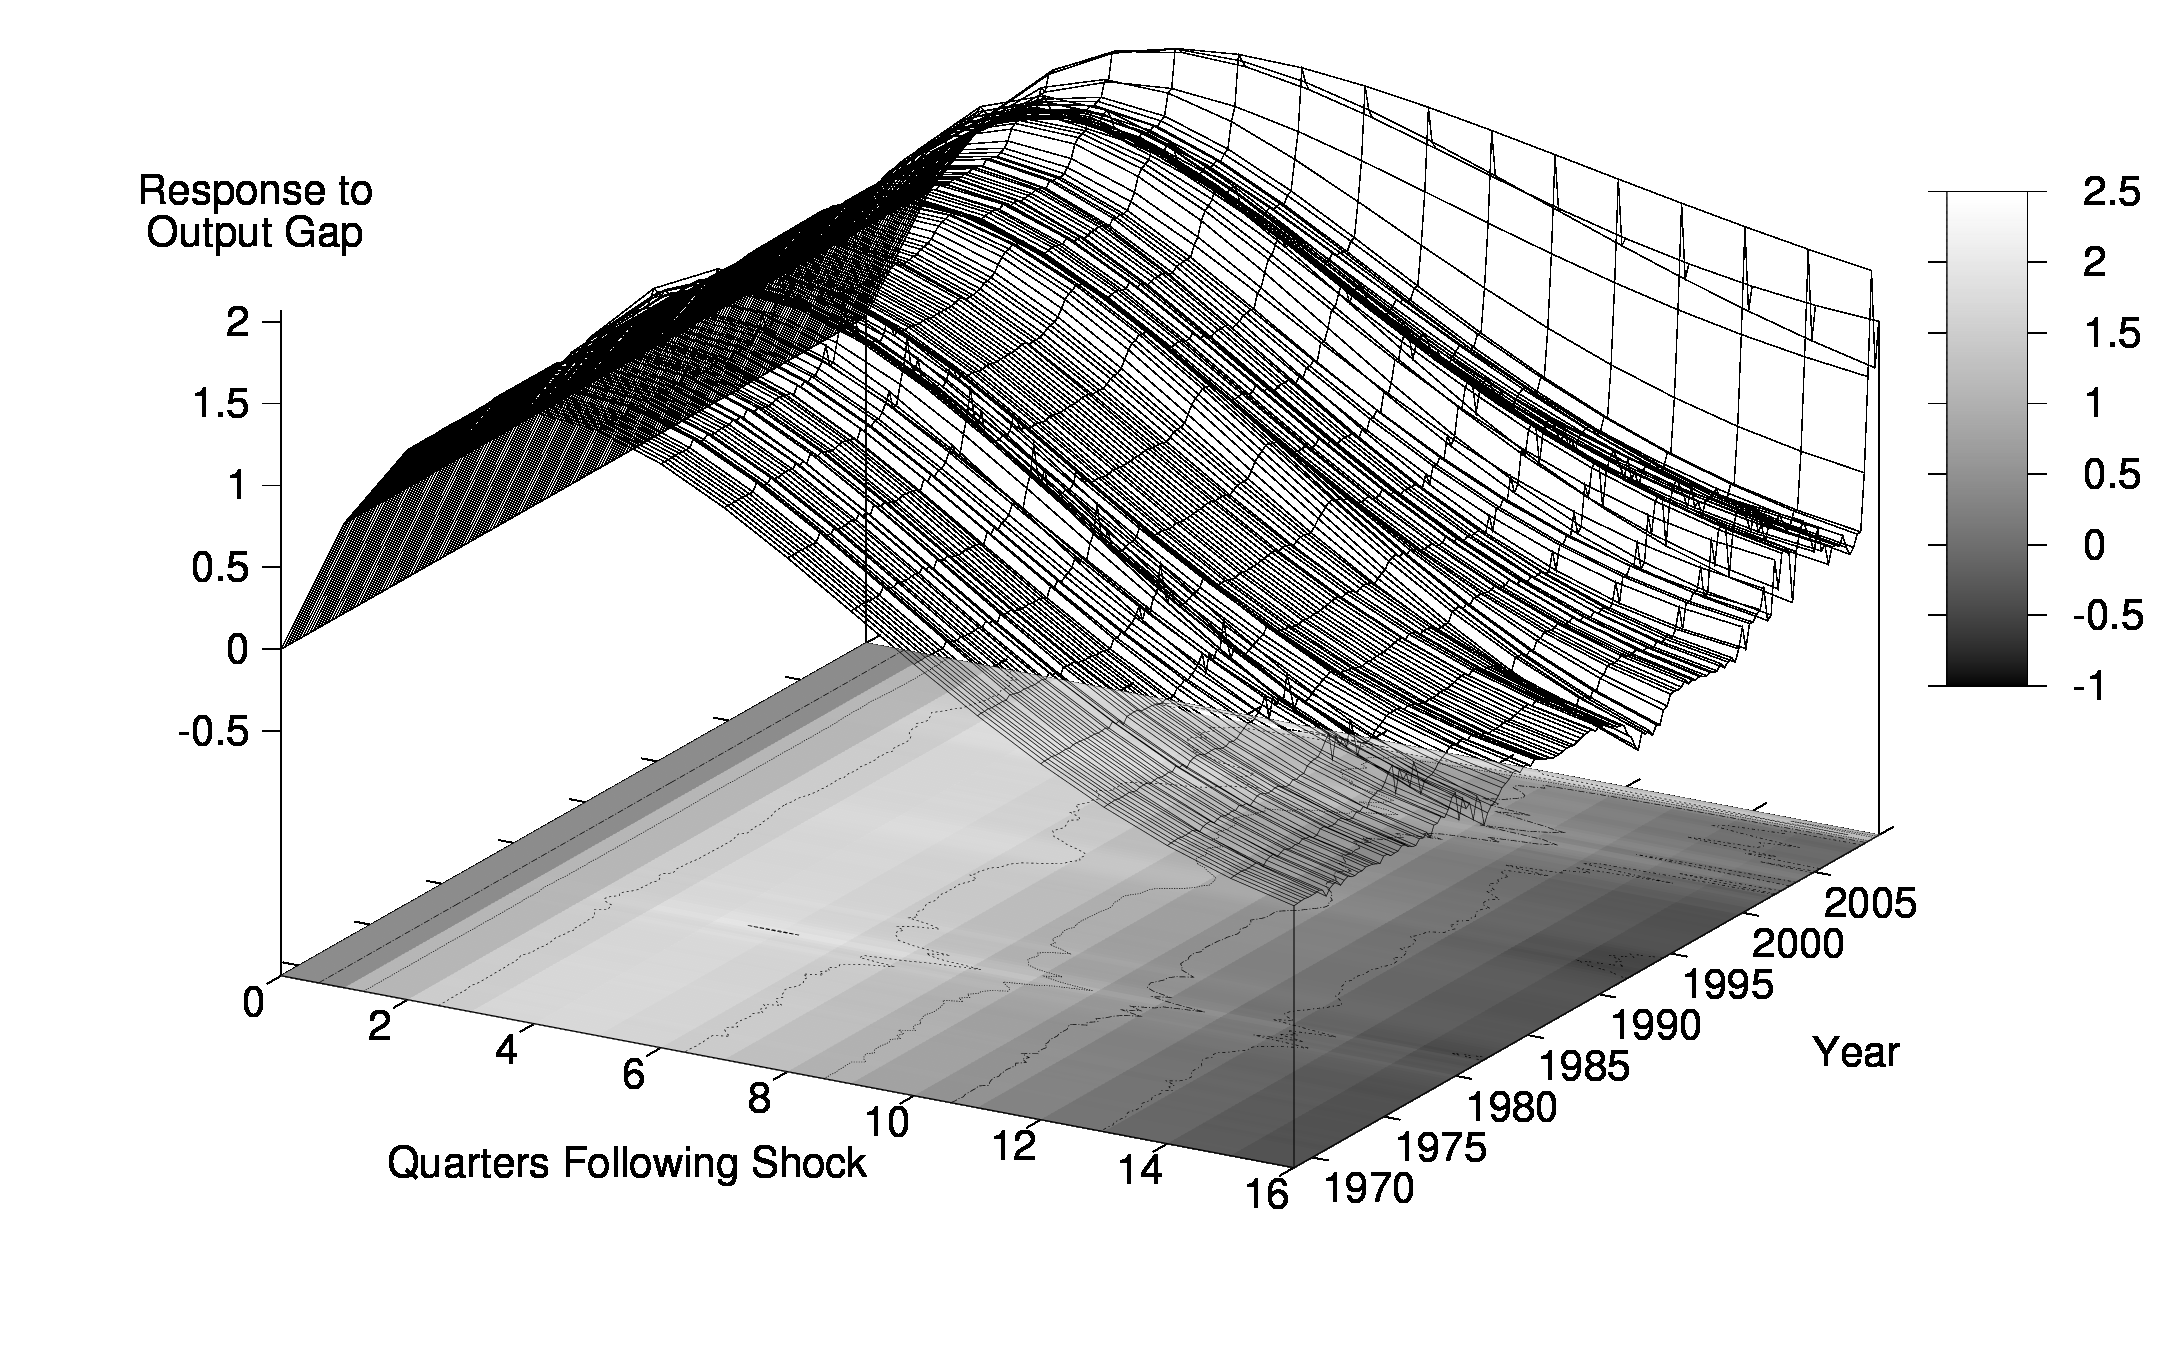
\includegraphics[width=1.9in,height=1.45in]{images/Irf16_Output_Gap_Output_Judgment_Shock.png} &
    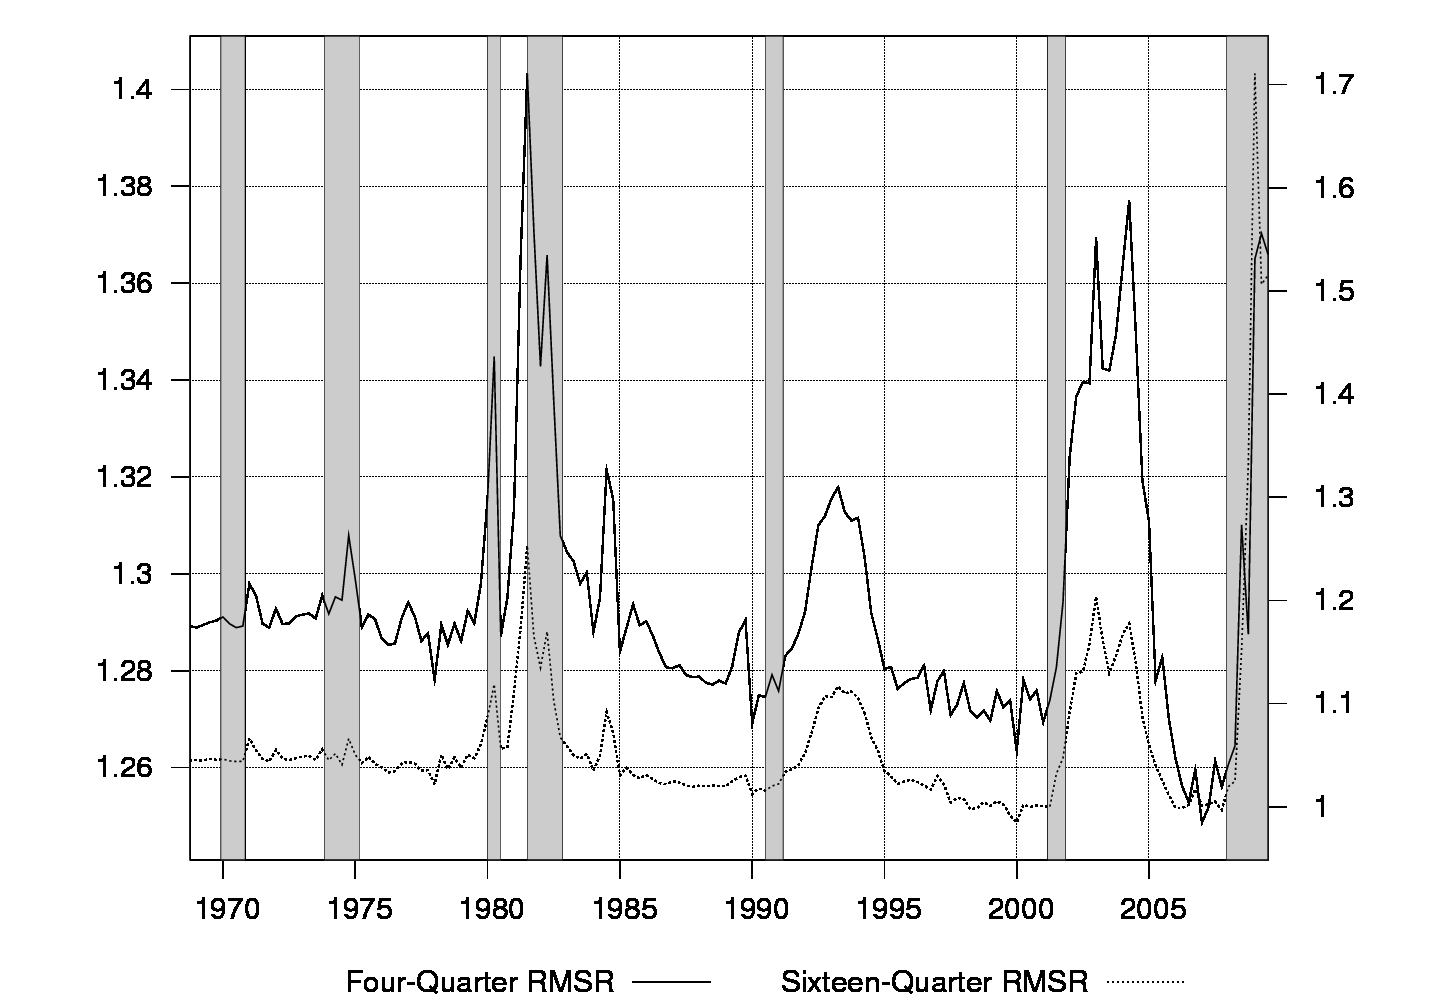
\includegraphics[width=1.9in,height=1.45in]{images/RMS16_Output_Gap_Output_Judgment_Shock.png} \\
    \end{tabular}
  \end{center}
  \end{block}

  \begin{block}{Comments}
    \small{
    \bi
    \item Output judgment shock increases output.
    \item Larger IRF's coincide with 1980s volatility, rapid growth of 1990s, slow growth in 2000s, slow recovery 2010 recession.
    \ei
    }
  \end{block}
}


\frame
{
  \ft{Impulse Responses: Output Judgment Shock}
  \begin{block}{Response to Inflation from Output Judgment Shock}
  \begin{center}
    \begin{tabular}{cc}
    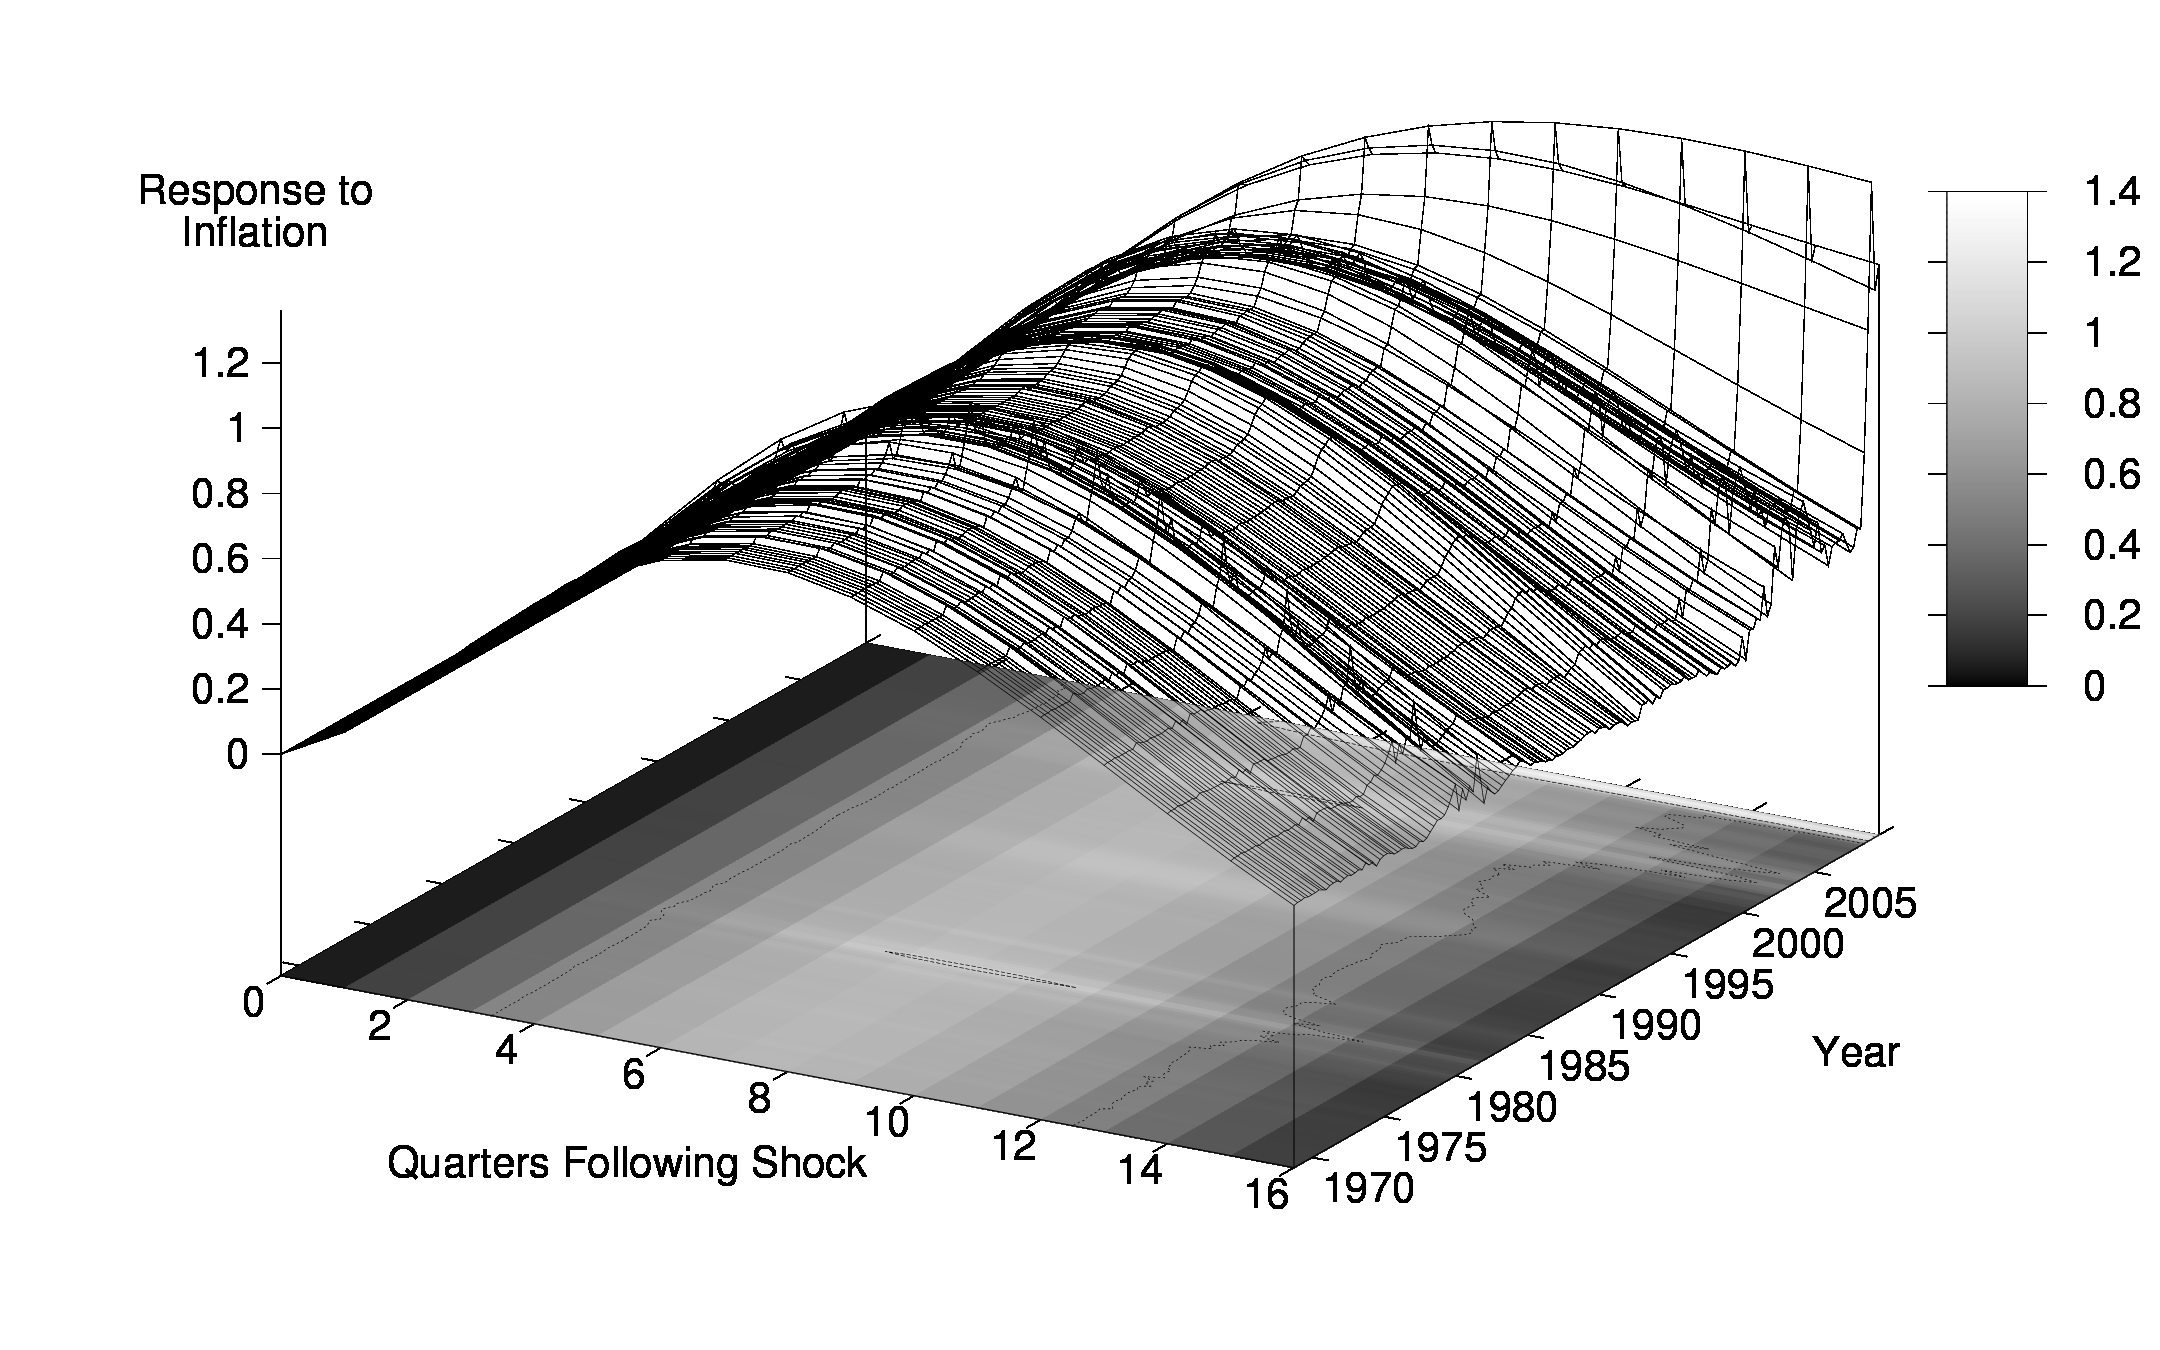
\includegraphics[width=1.9in,height=1.45in]{images/Irf16_Inflation_Output_Judgment_Shock.png} &
    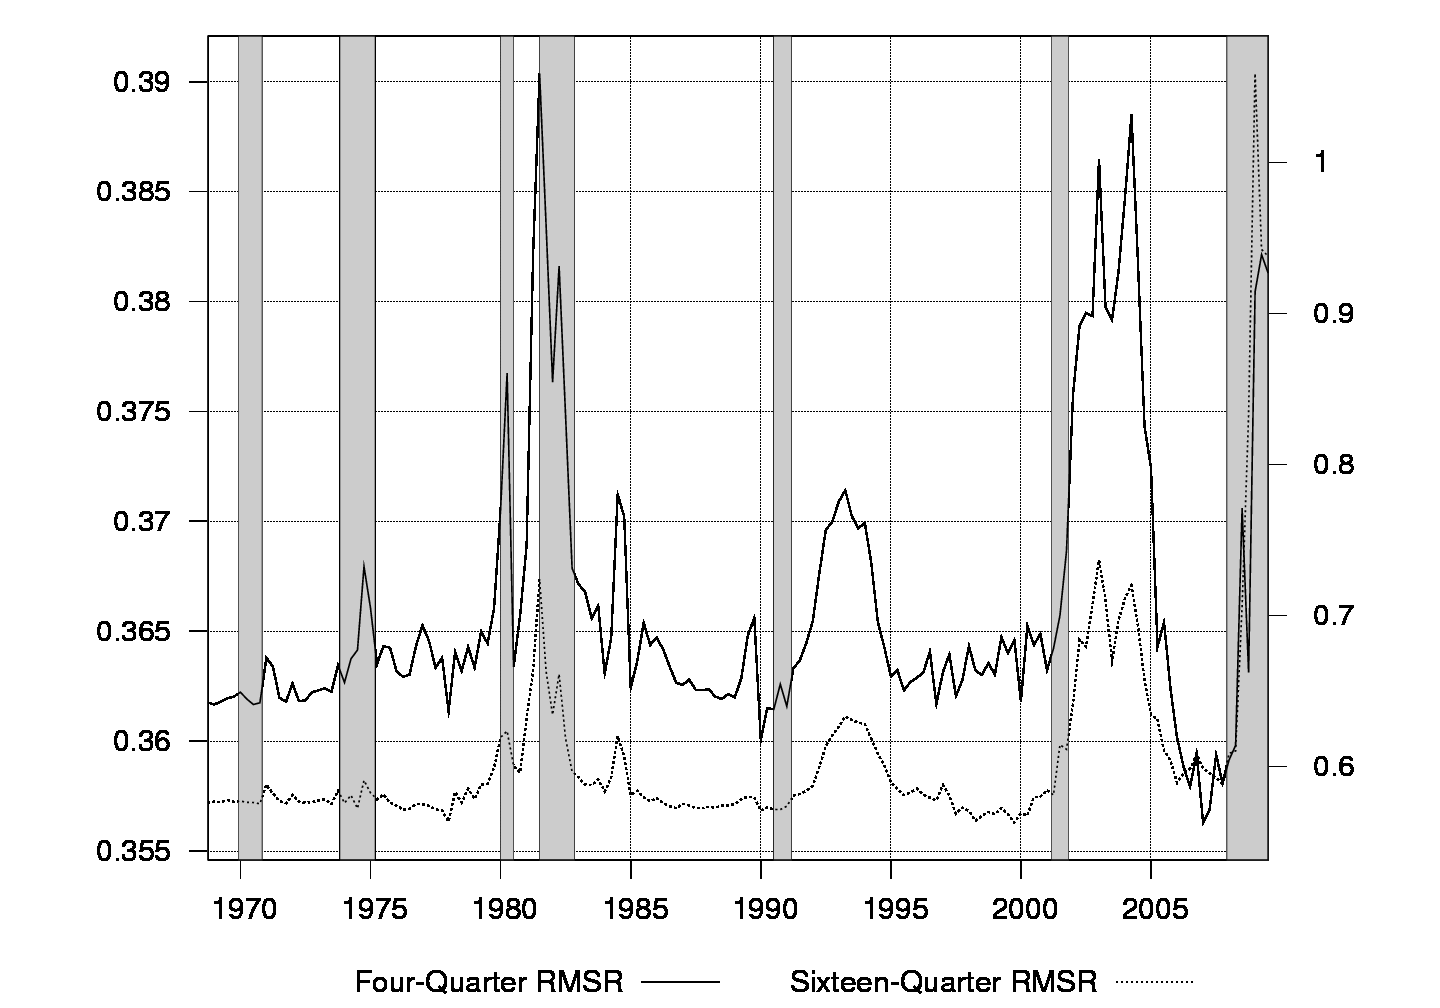
\includegraphics[width=1.9in,height=1.45in]{images/RMS16_Inflation_Output_Judgment_Shock.png} \\
    \end{tabular}
  \end{center}
  \end{block}

  \begin{block}{Comments}
    \small{
    \bi
    \item Output judgment shock increases inflation.
    \item Larger IRF's occur during same time periods.
    \ei
    }
  \end{block}
}

\frame
{
  \ft{Impulse Responses: Inflation Judgment Shock}
  \begin{block}{Response to Output Gap from Inflation Judgment Shock}
  \begin{center}
    \begin{tabular}{cc}
    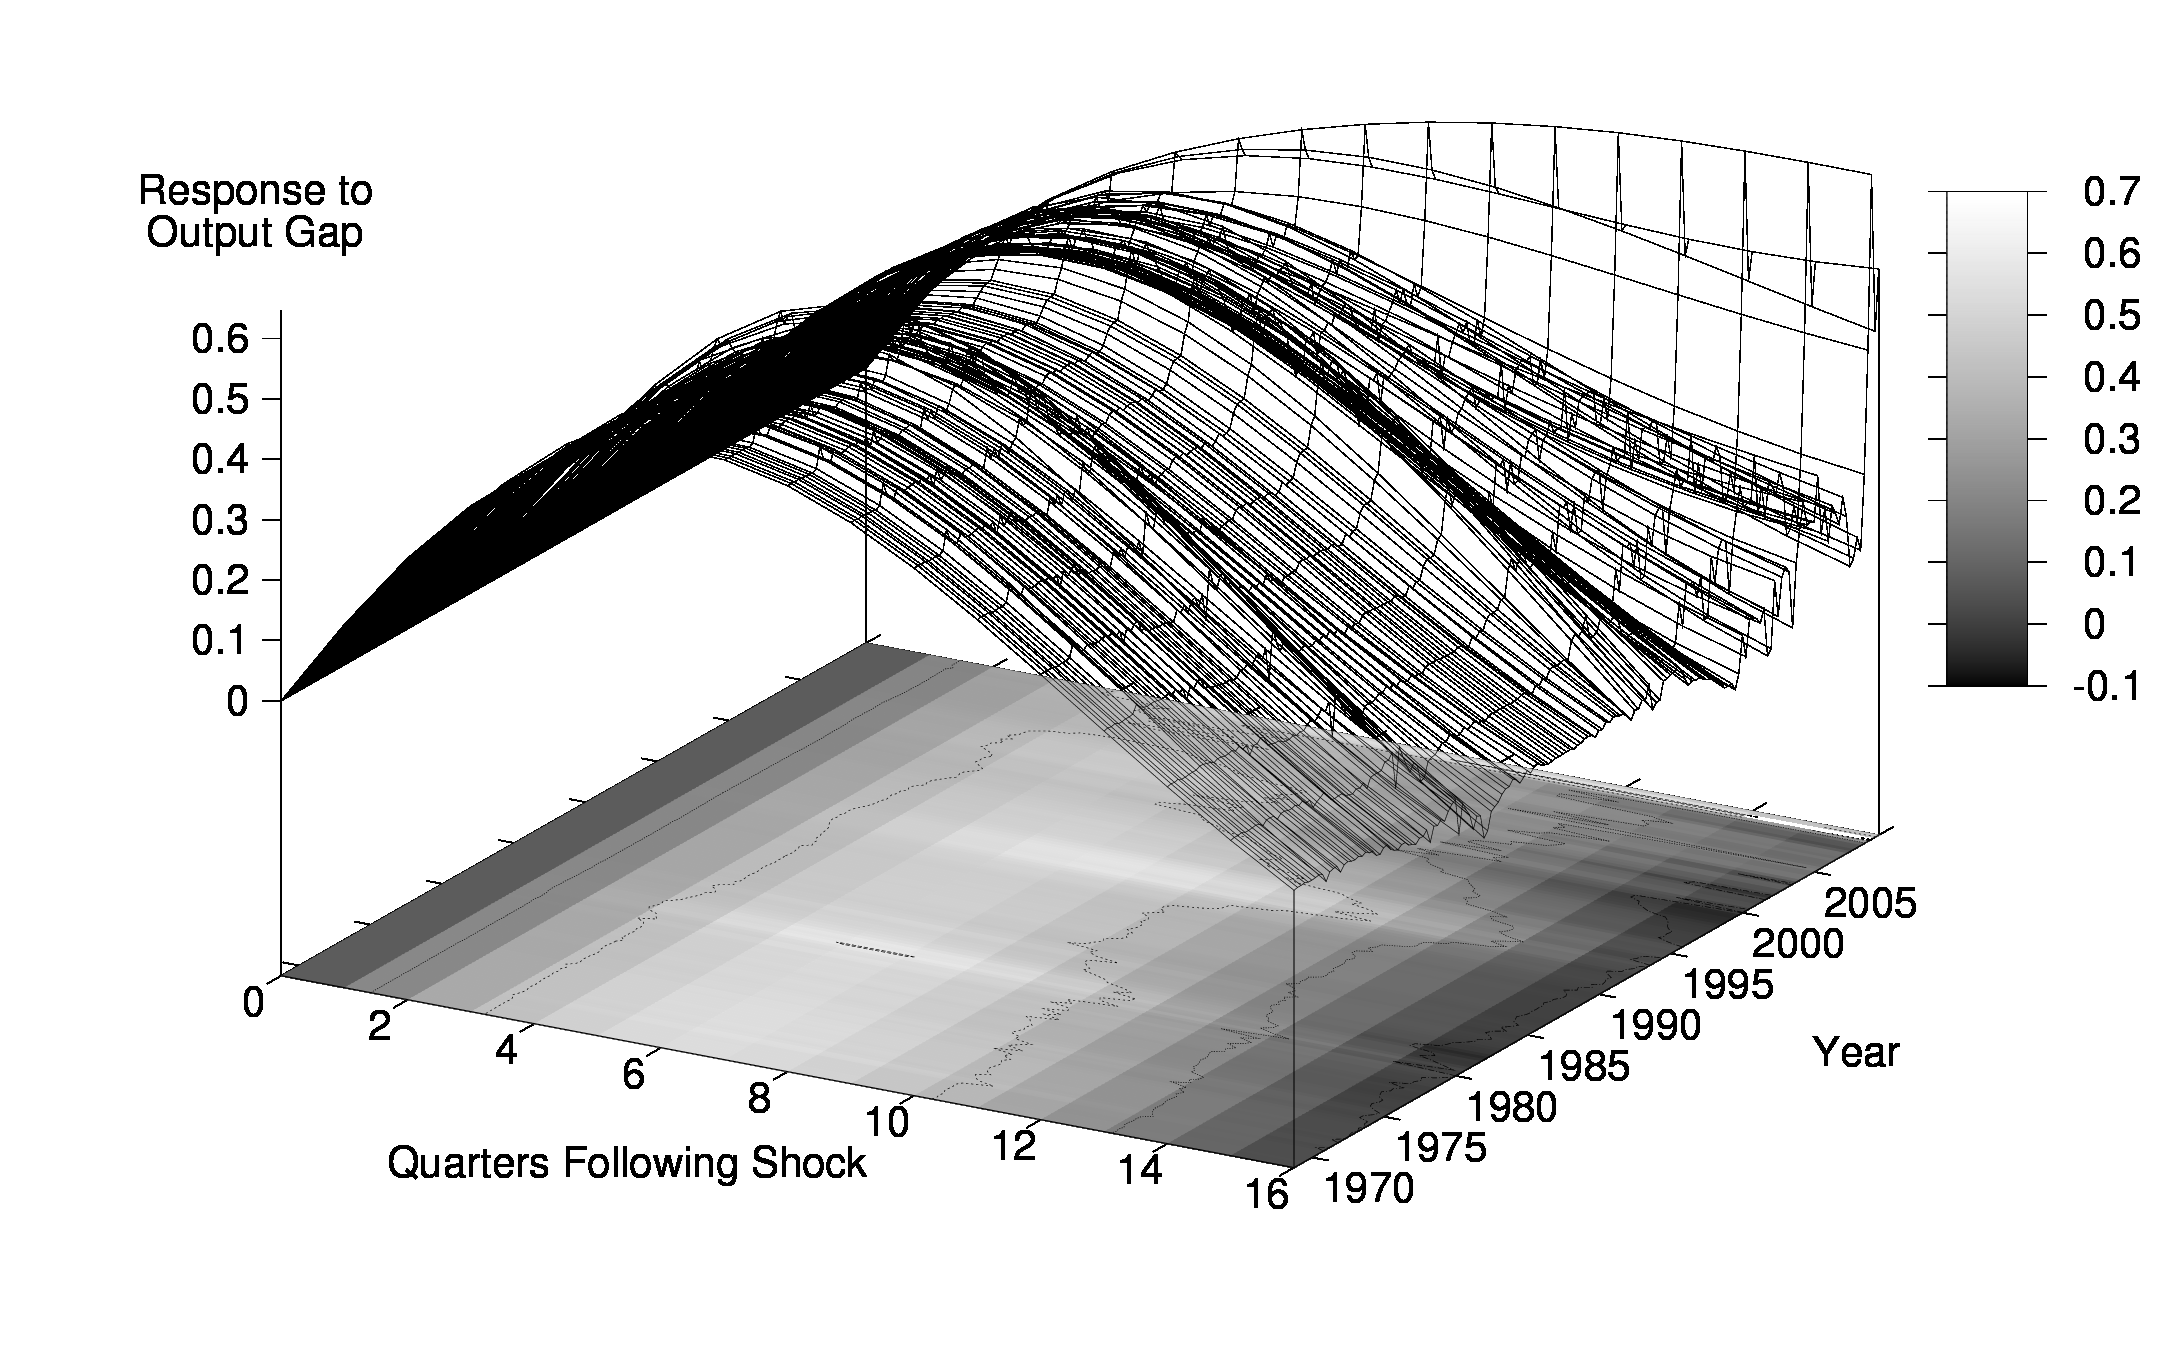
\includegraphics[width=1.9in,height=1.45in]{images/Irf16_Output_Gap_Inflation_Judgment_Shock.png} &
    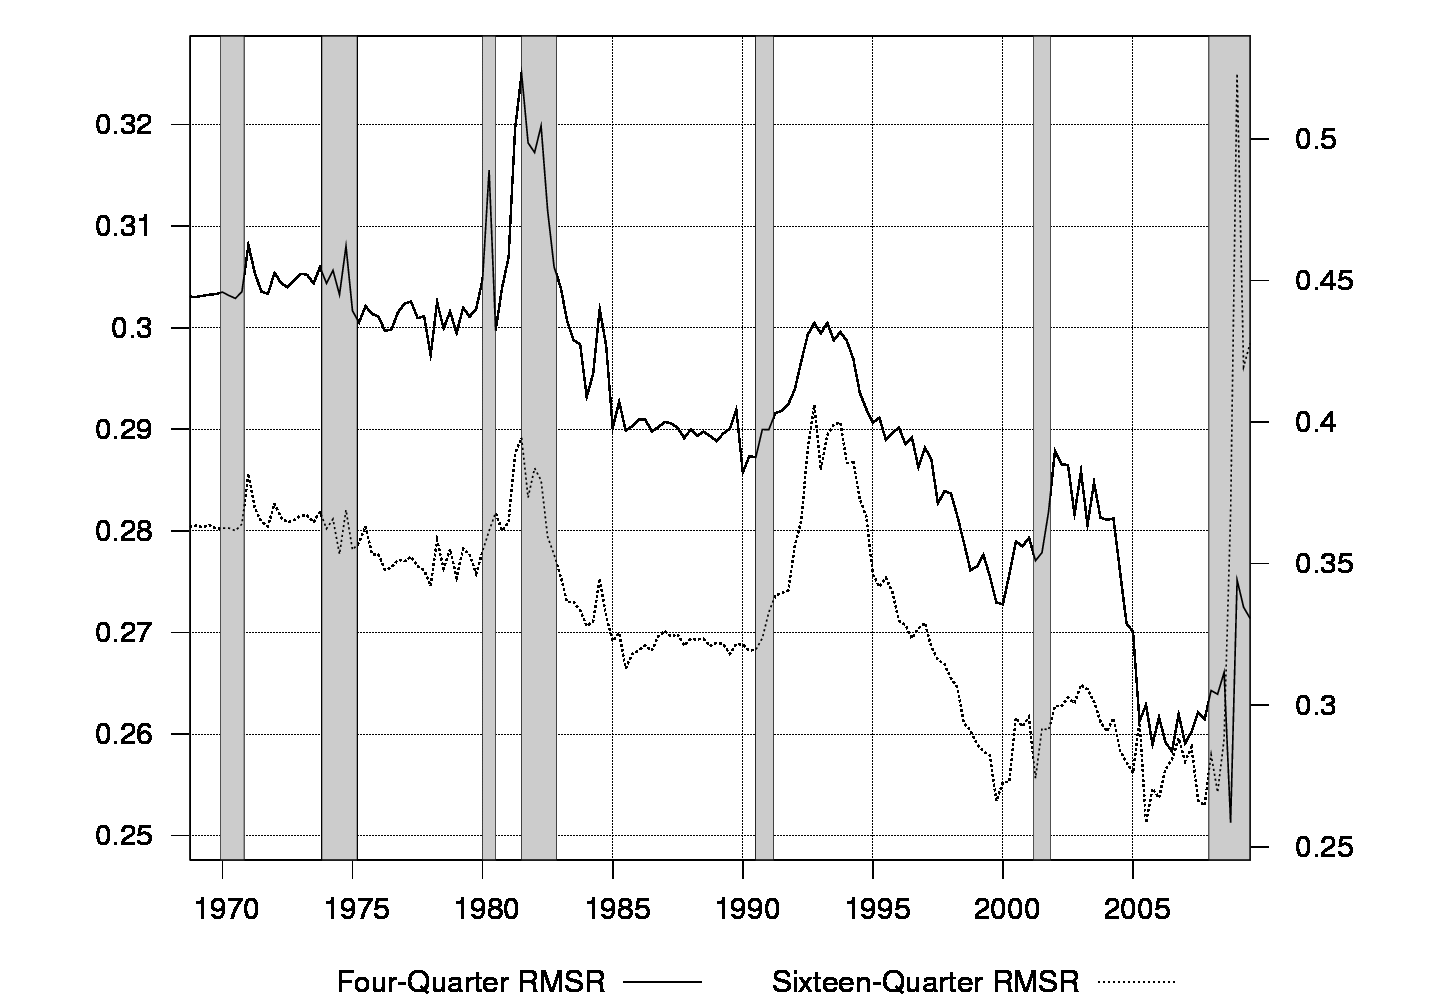
\includegraphics[width=1.9in,height=1.45in]{images/RMS16_Output_Gap_Inflation_Judgment_Shock.png} \\
    \end{tabular}
  \end{center}
  \end{block}

  \begin{block}{Comments}
    \small{
    \bi
    \item Inflation judgment shock increases output (reduces expected real interest rate).
    \item Inflation judgment IRFs on output have diminished over time.
    \ei
    }
  \end{block}
}


\frame
{
  \ft{Impulse Responses: Inflation Judgment Shock}
  \begin{block}{Response to Inflation from Inflation Judgment Shock}
  \begin{center}
    \begin{tabular}{cc}
    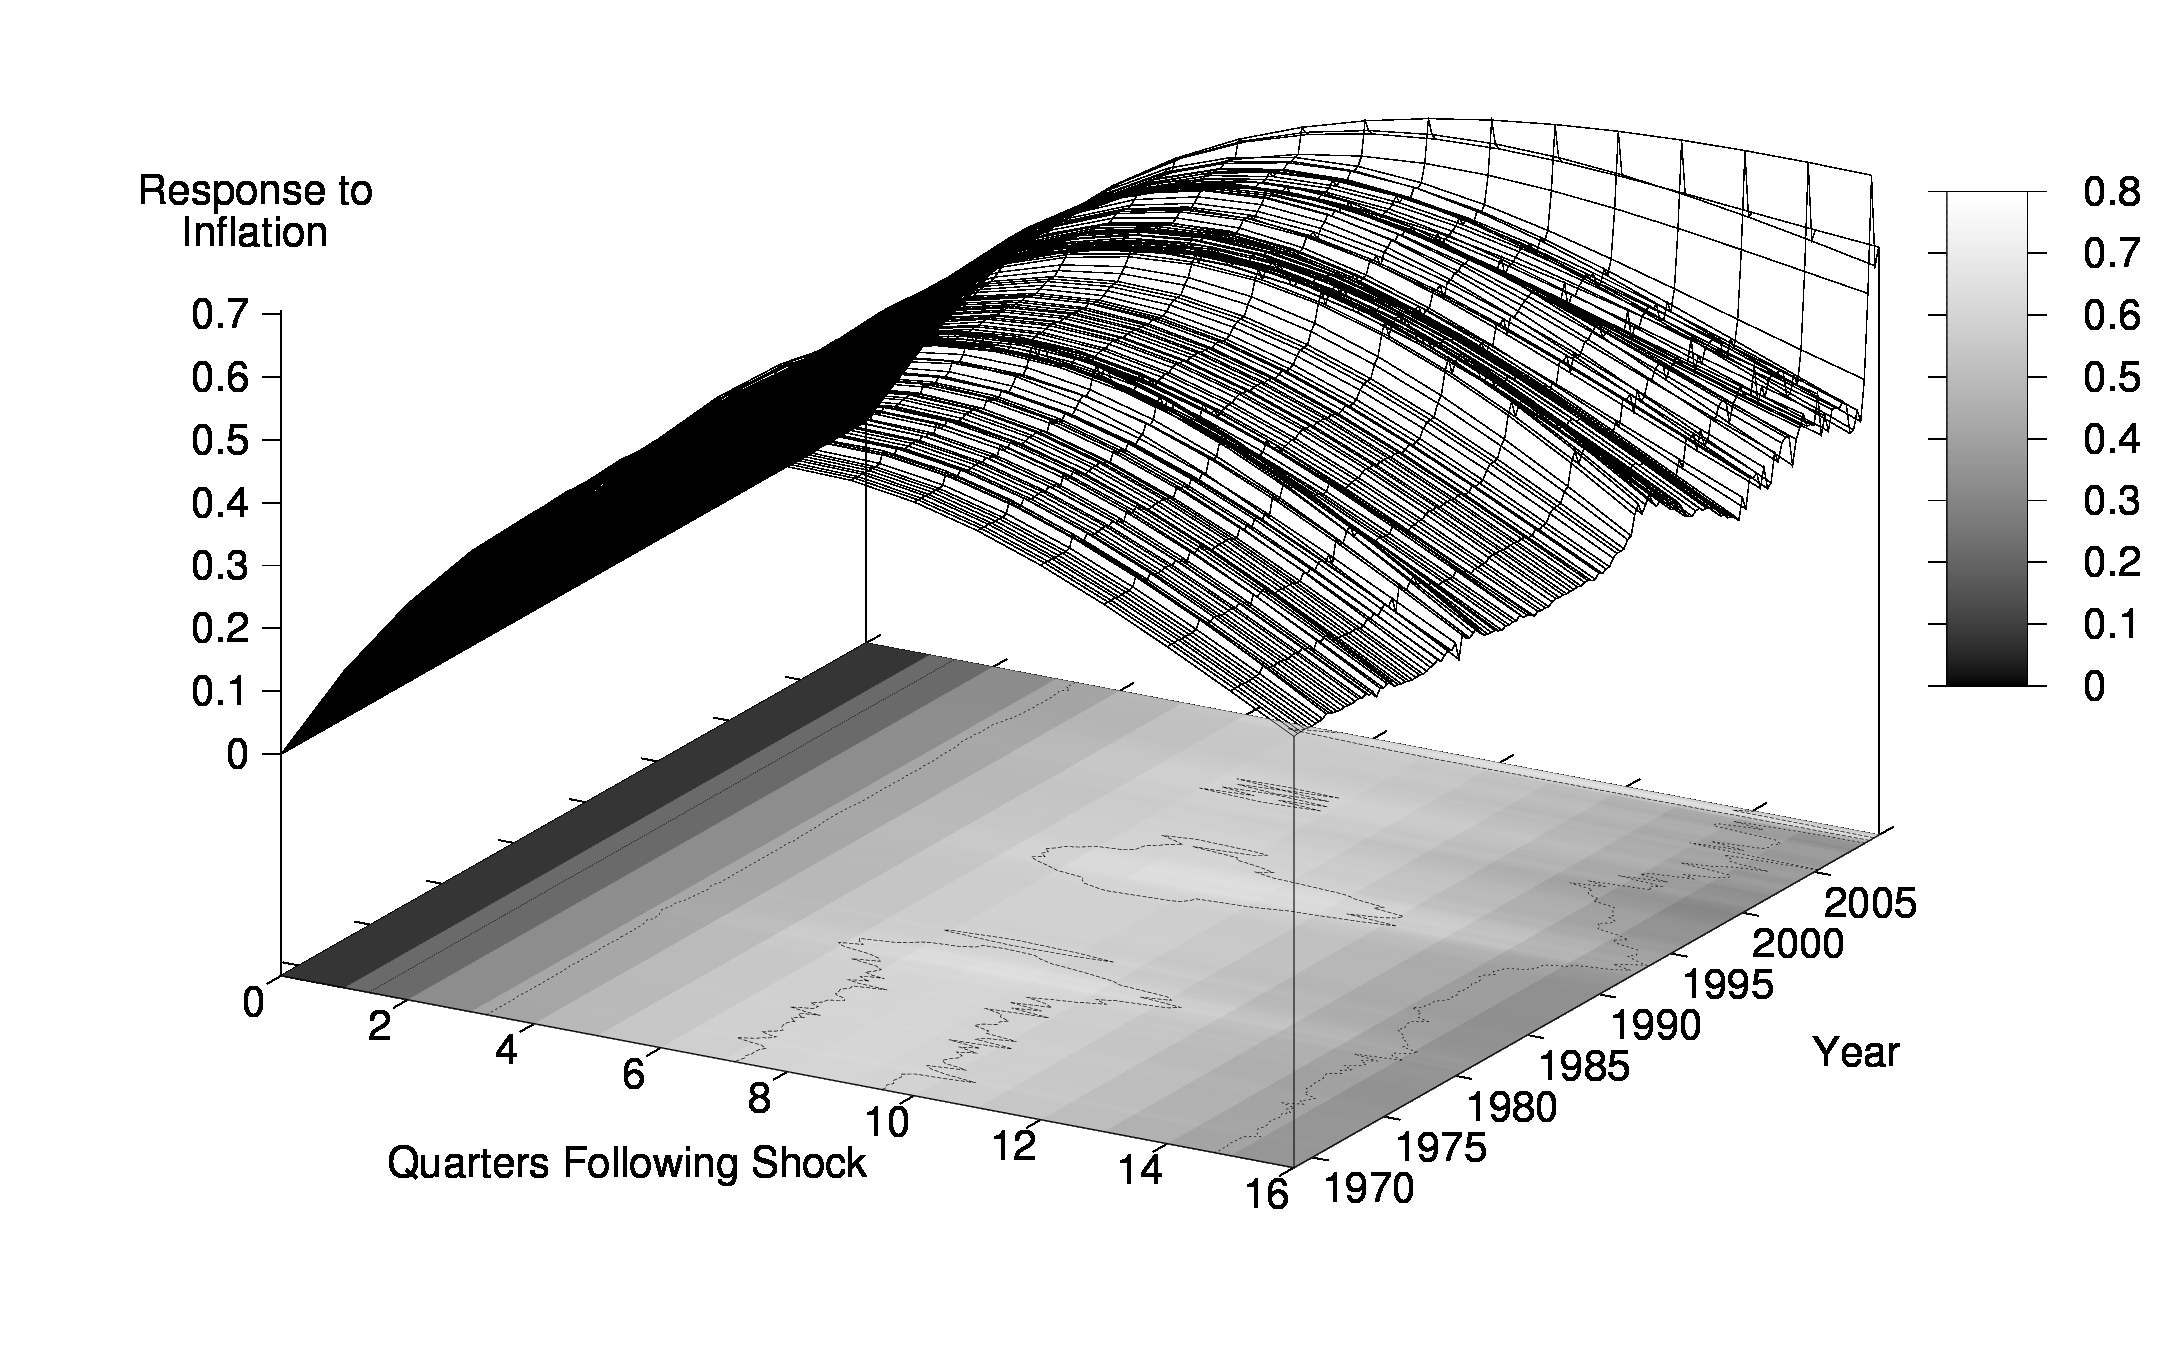
\includegraphics[width=1.9in,height=1.45in]{images/Irf16_Inflation_Inflation_Judgment_Shock.png} &
    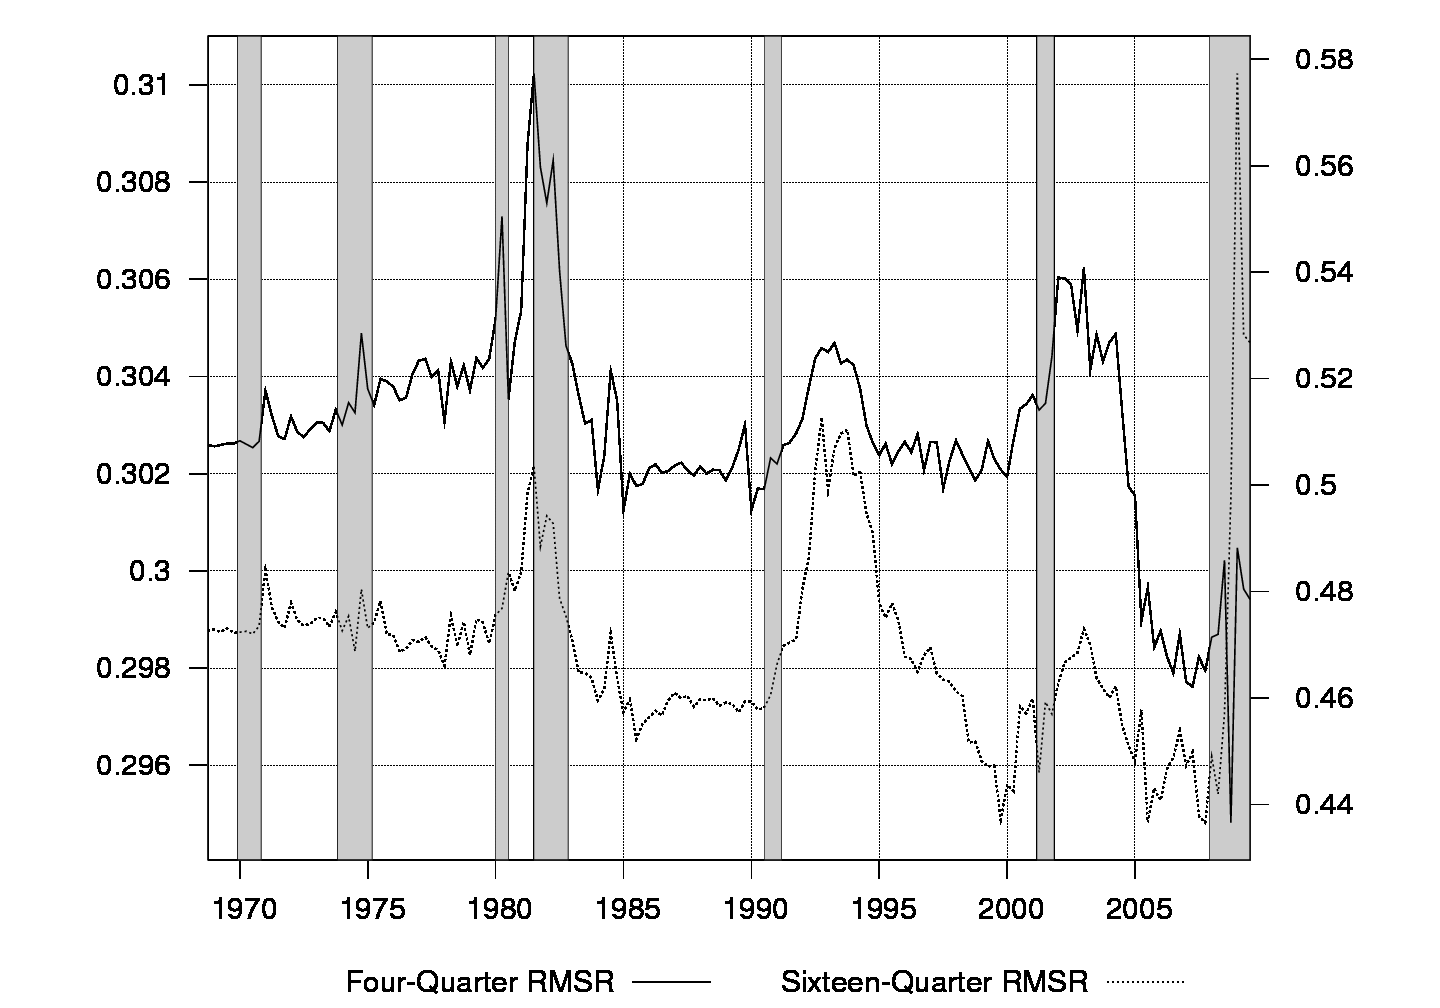
\includegraphics[width=1.9in,height=1.45in]{images/RMS16_Inflation_Inflation_Judgment_Shock.png} \\
    \end{tabular}
  \end{center}
  \end{block}

  \begin{block}{Comments}
    \small{
    \bi
    \item Inflation judgment shock increases inflation.
    \item Response is not symmetric over time.  Largest in last few years of the sample.
    \ei
    }
  \end{block}
}

\frame
{
  \ft{Comparing Impulse Responses}
  \begin{columns}
  \column[T]{2.5in}
  \begin{block}{Average Root Mean Squared Responses\\(One Std.Dev. Shock)} 
    \begin{footnotesize}
    \begin{tabular}{l|c|c}
      \multicolumn{3}{c}{First Four Periods of IRF} \\ \hline
      ~Shock & Output & Inflation \\ \hline 
      ~Natural Rate & 0.6018 & 0.1981  \\ 
      \only<3>{~\rowcolor{yellow}} Cost-Push & 0.1697 & 1.0864  \\ 
      ~Monetary Policy & 0.6364 & 0.1787  \\ 
      \only<2,4>{~\rowcolor{yellow}} Output Judgment & 1.2952 & 0.3662  \\ 
      \only<4>{~\rowcolor{yellow}} Inflation Judgment & 0.2911 & 0.3029  \\ 
      \hline
    \end{tabular}\\

    \begin{tabular}{l|c|c}
      \multicolumn{3}{c}{First Sixteen Periods of IRF} \\ \hline
      ~Shock & Output & Inflation \\ \hline 
      ~Natural Rate & 0.9918 & 0.6533 \\ 
      \only<3>{~\rowcolor{yellow}} Cost-Push & 0.1870 & 0.6953 \\ 
      ~Monetary Policy & 0.7742 & 0.4854 \\ 
      \only<2,4>{~\rowcolor{yellow}} Output Judgment & 1.0627 & 0.6060 \\ 
      \only<4>{~\rowcolor{yellow}} Inflation Judgment & 0.3353 & 0.4694 \\ 
      \hline
    \end{tabular}
    \end{footnotesize}
  \end{block}

  \column[T]{1.5in}
  \uncover<+->{
  \begin{block}{Comments}
    \begin{small}
    \bi
    \item<2> Output judgment shock has largest average impact on output.
    \item<3> Cost-push shock has largest impact on inflation.
    \item<4> Both output judgment and inflation judgment influence inflation dynamics.
    \ei
    \end{small}
  \end{block}
  }
  \end{columns}
}

\section{}
\subsection{Conclusion}
\frame
{
  \ft{Conclusions}
  \bi
  \item Judgment is a significant source of persistence for output and inflation.
  \item Inflation judgment is mostly dependent on stochastic disturbances.
  \item Output judgment is largely informed by concurrent natural rate shock.
  \item Both output and inflation judgment shocks are important drivers of business cycle fluctuations, along with natural rate shock and cost-push shock.
  \ei
}


\end{document}

